\documentclass[11pt]{article}
\usepackage[spanish, activeacute]{babel}
\usepackage[latin1]{inputenc}
\usepackage{amsmath, amssymb}
\usepackage{graphicx}
\usepackage{anysize}
\usepackage[a4paper=true]{hyperref}
\usepackage{caption}    
\title{Presence of the Virtual Observatory in the World}
\author{Jos\'{e} David Marroqu\'{i}n Toledo}
\date{13th of April, 2013}
\marginsize{3cm}{2cm}{0.5cm}{3cm}

\begin{document}
    \begin{center}
        \huge{\textbf{Presence of the Virtual Observatory in the World}}
    \end{center}
    \begin{center}
        \large{Jos\'{e} David Marroqu\'{i}n Toledo}

        \small{Federico Santa Mar\'{i}a Technical University}
    \end{center}

    \section{Abstract}
        This document publicizes the virtual observatories projects that make up
the International Virtual Observatory Alliance (IVOA), how they are distributed
worldwide and trough some brief descriptions, the tools which they themselves
develop under standards that facilitate the sharing of astronomical knowledge
and the interoperability. For this research were reviewed the website of the
IVOA and its membership, scientific publications, articles in book and other
electronics sources. This document is required by an initiative which intends
from Chile to development of an astro-informatics platform to manage and analyse
large-scale data based on the IVOA standards, project which involves the active
participation of university students of the Federico Santa Mar\'{i}a Technical
University.

    \section{Introduction}
        The Virtual Observatory (VO) is a international initiative which allows
the access to astronomical files and data centers to astronomers and any person
through Internet. With the standardization of the information and methods is
possible study the astronomical data without the physical requirement of the
tools and location.\\

        In June 2002, was made the International Virtual Observatory Alliance
(IVOA) to ``facilitate the international coordination and collaboration
necessary for the development and deployment of the tools, systems and
organizational structures necessary to enable the international utilization of
astronomical archives as an integrated and interoperating virtual observatory''.
Actually, the IVOA is composed of 19\footnote{On the official website in
\textbf{What is the IVOA} ``the IVOA now comprises 17 VO projects'', but in
\textbf{Member Organizations} appears 19 members listed.} projects of America,
Asia, Europa and Oceania; its members meet two times each year in
Interoperability  Workshops to have discussions face-to-face and resolve
technical questions.\\

        An initiative led by Ph. D. Mauricio Solar alongisde students of
Federico Santa Mar\'{i}a Technical University intends to develop an
astro-informatics platform to manage and analyse intelligently large-scale data
based on the IVOA standards. Due the above, this document aims:

        \begin{itemize}
            \item Publicize the distribution of the virtual observatories
worldwide.
            \item List the tools developed by the virtual observatories and
their status from the information provided on their official websites on
Internet.
            \item Get an idea about what additional tools could be developed to
guarantee fulfilling the main objective\footnote{\textit{``Desarrollo de una
plataforma astro-inform\'{a}tica para la administraci\'{o}n y an\'{a}lisis
inteligente de datos a gran escala''} according to the name of Fondef D11$ \vert
$1060 project}.
        \end{itemize}

        For these purposes were reviewed the official websites of the IVOA and its
members, were read sections of documents about virtual observatories like
``Virtual Observatories, Data Mining, and Astroinformatics'' of Kirk Borne,
George Mason University, among others.\\
        
    \section{Distribution of IVOA Virtual Observatories Worlwide and its
Projects}
        \subsection{The IVOA}
            From June 2002, projects of virtual observatories have come to
integrate the International Virtual Observatory Alliance (IVOA) under the
\textbf{Guidelines for Participation\footnote{The guidelines are available in a
paper in PDF and DOC format from
\url{http://www.ivoa.net/documents/latest/IVOAParticipation.html}}}. These were
founded through national and international governmental and private programs in
collaboration with various centers of scientific studies, universities and
others. Who integrate this project, the Virtual Observatory (VO), share
knowledge between them and the community in a standardized manner. They
themselves are who develop these standards for data exchange and
interoperability.\\

            The table 1 shows the partners of IVOA to May 2013.\\

            \begin{center}
                \begin{tabular}{|p{7cm} | p{7cm}|}
                    \hline
                    \textbf{Project} & \textbf{URL} \\
                    \hline
                    Argentina Virtual Observatory &
\url{http://nova.conicet.gov.ar/} \\
                    \hline
                    Armenian Virtual Observatory &
\url{http://www.aras.am/Arvo/arvo.htm} \\
                    \hline
                    AstroGrid & \url{http://www.astrogrid.org/} \\
                    \hline
                    Australian Virtual Observatory & \url{http://aus-vo.org.au/}
\\
                    \hline
                    Brazilian Virtual Observatory &
\url{http://www.lna.br/bravo/} \\
                    \hline
                    Canadian Virtual Observatory &
\url{http://www.china-vo.org/} \\
                    \hline
                    Chinese Virtual Observatory &
\url{http://www.cadc-ccda.hia-iha.nrc-cnrc.gc.ca/cvo/} \\
                    \hline
                    European Space Agency &
\url{http://www.sciops.esa.int/index.php?project=ESAVO} \\
                    \hline
                    European Virtual Observatory & \url{http://www.euro-vo.org/}
\\
                    \hline
                    German Astrophysical Virtual Observatory &
\url{http://www.g-vo.org/} \\
                    \hline
                    Hungarian Virtual Observatory & \url{http://hvo.elte.hu/en/}
\\
                    \hline
                    Italian Virtual Observatory & \url{http://vobs.astro.it/} \\
                    \hline
                    Japanese Virtual Observatory & \url{http://jvo.nao.ac.jp/}
\\
                    \hline
                    Observatorie Virtual France &
\url{http://www.france-vo.org/} \\
                    \hline
                    Russian Virtual Observatory &
\url{http://www.inasan.rssi.ru/eng/rvo/} \\
                    \hline
                    Spanish Virtual Observatory &
\url{http://svo.cab.inta-csic.es/} \\
                    \hline
                    Ukranian Virtual Observatory & \url{http://www.ukr-vo.org/}
\\
                    \hline
                    Virtual Astronomical Observatory &
\url{http://www.usvao.org/} \\
                    \hline
                    Virtual Observatory India &
\url{http://vo.iucaa.ernet.in/~voi/} \\
                    \hline
                \end{tabular}

            Table 1. IVOA Partners.
            \end{center}

            Almost half of IVOA virtual observatories are supported in Europe: 9
of the total; 1 belong to Oceania, 4 to America and 5 to Asia\footnote{As the
mayor part of Rusia's territory is in Asia, it will be considered like a virtual
observatory of Asian continent.}. The figure 1 shows the distribution of the
IVOA's membership per continent.\\

            \begin{figure}[h]
                \begin{center}
                    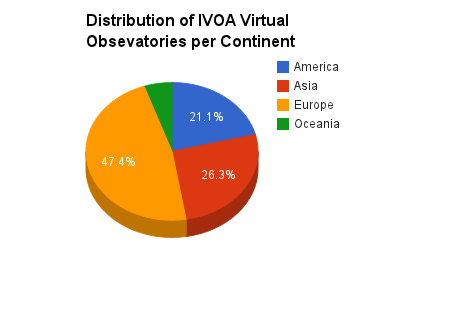
\includegraphics[width=110mm]
{IVOA_VOs_distribution_per_continent_by_JDMT.png}
                    \caption{International Virtual Observatory Alliance
distribution per continent.}
                \end{center}
            \end{figure}

            If Chile became part of International Virtual Observatory Alliance,
the distribution of the members per continent will be as shown in the figure
2.\\

            \begin{figure}[h]
                \begin{center}
                    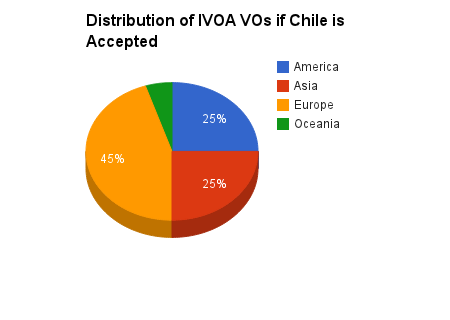
\includegraphics[width=110mm]
{if_Chile_is_Accepted_by_JDMT.png}
                    \caption{International Virtual Observatory Alliance
distribution per continent if Chile is accepted.}
                \end{center}
            \end{figure}

            Without considering the status of the internal projects of the
virtual observatories, the membership of Chile would contribute to the
cooperation, development and interoperability from America in the same percent
that Asia.  Furthermore, this fact would be very significant, because a large
numbers of astronomical centers like observatories are placed in this country.
For now, is intended to work with a certain quantity of data of ALMA.\\

    \section{List of IVOA Virtual Observatories}
        \subsection{America}
            \subsubsection{Brazilian Virtual Observatory (BRAVO)}
            The BRAVO was born with the Declarations of Intentions signed on
18th of August, 2008 by six research institutes and the Brazilian Astronomical
Societyi (SBA, in its Portuguese acronym). Later, the Brazilian Virtual
Observatory was founded by the National Institute for Science and Technology in
Astrophysics (INCT-A, in its Portugese acronym).

                \begin{itemize}
                    \item \textbf{Projects}
                        \begin{itemize}
                            \item BRAVO@IAG
                            \item BRAVO@INPE
                                \begin{itemize}
                                    \item \textbf{Description\footnote{On the
\textbf{List of IVOA Virtual Observatories} section, a brief description of each
proyect appears only if was found some information of them in the sources.}:}
generate investment in information technology on Computational Infraestructure,
Data Grid, Data Processing and Data Mining.
                                \end{itemize}
                            \item BRAVO@LNA
                                \begin{itemize}
                                    \item \textbf{Description:} making of a
virtual observatory dedicated to Southern Astrophysical Research Telescope
(SOAR) data from Brazilian astronomers.  \end{itemize}
                            \item BRAVO@UFSC
                                \begin{itemize}
                                    \item \textbf{Description:} researching of
the of the power spectral synthesis as a mean to estimate the physical
properties of the galaxies.
                                \end{itemize}
                            \item CYCLOPS
                                \begin{itemize}
                                    \item \textbf{Description:} software which
models the optical emission from AM Her systems including the four Stokes
parameters.
                                \end{itemize}
                        \end{itemize}
                \end{itemize}

            \subsubsection{Canadian Virtual Observatory (CVO)}
                \begin{itemize}
                    \item \textbf{Projects}
                        \begin{itemize}
                            \item Data Sharing (VOSpace 2.0)
                                \begin{itemize}
                                    \item \textbf{Description:} a service which
allows users to share files and collaborate with team members. 
                                \end{itemize}
                            \item Table Access Protocol (TAP-1.0)
                                \begin{itemize}
                                    \item \textbf{Description:} a service which
allows the access to all the data described by the Common Archive Observation
Model (CAOM) in use at the CADC and tables from other projects.
                                \end{itemize}
                            \item Observation Model Core Components
(ObsCore-1.0)
                                \begin{itemize}
                                    \item \textbf{Description:} a model which
implements a standard view for \textbf{Table Access Protocol (TAP-1.0)}.
                                \end{itemize}
                            \item Simple Image Access (SIA-1.0)
                                \begin{itemize}
                                    \item \textbf{Description:} a SIA-1.0
compliant query service for easy access to calibrated images from most our data
collections.
                                \end{itemize}
                        \end{itemize}
                \end{itemize}

            \subsubsection{Nuevo Observatorio Virtual Argentino (NOVA)}
                The NOVA was founded by eight institutions\footnote{The
institutions which founded the NOVA are the Observatorio Astron\'{o}mico de
C\'{o}rdova (OAC), Facultad de Ciencias Astron\'{o}micas y Geof\'{i}sicas de La
Plata/Universidad de Nacional de la Plata (FCAGLP/UNLP), the Instituto de
Astrof\'{i}sica de La Plata (IALP), the Instituto Argentino de
Radioastronom\'{i}a (IAR), the Instituto de Astronom\'{i}a y F\'{i}sica del
Espacio (IAFE), the Instituto de Ciencias Astron\'{o}micas, de la Tierra y del
Espacio (ICAFE), the Instituto de Astronom\'{i}a Te\'{o}rica y Experimental
(IATE), and the Complejo Astron\'{o}mico El Leoncito (CASLEO).} among which
important astronomical institutes and the National University of La Plata
through the Faculty of Astronomical Sciences and Geophysics of La Plata. It was
born in January 2009. From June 2013, the NOVA will begin its operations and
intends, in addition to provide the astronomical observations from its official
website, to implement a platform web where it can work with the
data\footnote{Agencia CTyS. (2013, May 9). Instituciones astron\'{o}micas lanzan
el Nuevo Observatorio Virtual Argentino. \textit{Agencia CTyS}. Retrieved from:
\url{http://www.ctys.com.ar/index.php?idPage=20&idArticulo=2585}}.

    \begin{itemize}
        \item \textbf{Projects}
            \begin{itemize}
                \item NOVA@CASLEO
                \item NOVA@IAFE
                    \begin{itemize}
                        \item \textbf{Description:} building a database for the
observations\footnote{The more than 6 terabytes of date was stored in CDs and
DVDs.} reached by the HASTA solar telescope and its applications.
                    \end{itemize} 
                \item NOVA@IALP
                \item NOVA@IAR
                \item NOVA@IATE
                \item NOVA@ICATE
                    \begin{itemize}
                        \item \textbf{Description:} building a database for the
spectroscopic observations\footnote{Until 1987, the database was stored in
photographic plates. After that year, the information was stored in CDs and
DVDs.} available at ICATE.
                    \end{itemize}
                \item NOVA@OAC
                \item NOVA@FCAGLP
            \end{itemize}
        \end{itemize}

            \subsubsection{US Virtual Astronomical Observatory (VAO)}
                The VAO is the succesor of the NVO (National Virtual
Observatory) and was founded by the NSF and the NASA and. It is in charge of the
VAO, LLC, an entity created by the Associated Universities, Inc. (AUI) and the
Association of Universities for Research in Astronomy (AURA). VAO advise the VAO
Science Council \footnote{\url{http://www.usvao.org/governance/}}. The US VO is
a co-founder of the IVOA.

                \begin{itemize}
                    \item \textbf{Projects}
                        \begin{itemize}
                            \item Data Discovery Tool
                                \begin{itemize}
                                    \item \textbf{Description:} 
                                \end{itemize}
                            \item Iris: SED Analysis Tool
                                \begin{itemize}
                                    \item \textbf{Description:} 
                                \end{itemize}
                            \item Cross-Comparision Tool
                                \begin{itemize}
                                    \item \textbf{Description:} 
                                \end{itemize}
                            \item Time Series Search Tool
                                \begin{itemize}
                                    \item \textbf{Description:} 
                                \end{itemize}
                        \end{itemize}
                \end{itemize}

        \subsection{Europe}
            \subsubsection{Armenian Virtual Observatory (ArVO)}
                The ArVo is based on the Digital First Byukaran Survey (DFBS), a
project between Byurakan Astrophysical Observatory, Armenia; ``La Sapienza''
Universit\`{a} di Roma, Italia; Cornell University, USA and
VO-France\footnote{Mickaelian, A., Sargsyan, L., Gigoyan, K., Erastova, L.,
Sinamyan, P., Hovhannisyan, L., ...Mykayelyan, G. (2007, December). Science with
the Armenian Virtual Observatory (ArVo).  Retrieved from
\url{http://www.grid.am/pdf/Science_with_the_Armenian_Virtual_Observatory_(ArVO).pdf}}.
Its virtual observatory was launched in February 2008\footnote{Armenian
News-NEWS.am. (2012, February 18). Armenia creates virtual observatory server.
\textit{NEWS.am}. Retrieved from \url{http://news.am/eng/news/93843.html}}.

                \begin{itemize}
                    \item \textbf{Projects}
                \end{itemize}

            \subsubsection{Hungarian Virtual Observatory (HVO)}
                \begin{itemize}
                    \item \textbf{Projects}
                \end{itemize}

            \subsubsection{AstroGrid}
                The AstroGrid is the United Kingdom's virtual observatory. It
began as a project in 2001 and was launched in April 2008 along its working
service and user software. It has been financed by the Particle Physics and
Astronomy and Research Council (PPARC) and the Science \& Technology Facilities
Council (STFC).

                \begin{itemize}
                    \item \textbf{Projects}
                        \begin{itemize}
                            \item Topcat
                                \begin{itemize}
                                    \item \textbf{Description:} an interactive
graphical viewer and editor for tabular data for formats like FITS and VOTable.
                                \end{itemize}
                            \item VODesktop
                                \begin{itemize}
                                    \item \textbf{Description:} an analysis
tools wich allows limit the choice of resources through specific data saving.
                                \end{itemize}
                            \item AstroRuntime
                                \begin{itemize}
                                    \item \textbf{Description:} an API
implemented in JAVA wich facilitates the access to the \textbf{VODesktop}
services from almost any programming language \footnote{On the AstroGrid's
official website there is a document about how access VODesktop using Python
script at \url{http://www.astrogrid.org/agpython.html}}. 
                                \end{itemize}
                        \end{itemize}
                \end{itemize}

            \subsubsection{European Space Agency Virtual Observatory (ESA-VO)}
                \begin{itemize}
                    \item \textbf{Projects}
                \end{itemize}

            \subsubsection{European Virtual Observatory (EURO-VO)}
                \begin{itemize}
                    \item
                \end{itemize}

            \subsubsection{German Astrophysical Virtual Observatory (GAVO)}
                The GAVO was launched in 2003\footnote{Its first publications
dates from 2003. In 2004, H. Adorf and GAVO Team talking about ``GAVO - after
one year'' at the Astronomical Data Analysis (ADA) III Sant'Agata sui due Golfi,
Italy. The birth of this VO is inferred from the above.}. It is financed through
the Federal Ministry of Education and Research (BMBF).
                 
                \begin{itemize}
                    \item \textbf{Projects}
                        \begin{itemize}
                            \item GAVO Data Center
                                \begin{itemize}
                                    \item \textbf{Description:} A growing
collection of data and services provided on behalf of third parties. Some of the
GAVO services are also available on \url{http://dc.zah.uni-heidelberg.de/}
                                \end{itemize}
                            \item GAVO Data Center
                                \begin{itemize}
                                    \item \textbf{Description:} a collection of
data and services on behalf of third parties. 
                                \end{itemize}
                            \item MPA Simulations access
                                \begin{itemize}
                                    \item \textbf{Description:} a web service
for querying the results of the Millennium simulation using SQL.
                                \end{itemize}
                            \item MultiDark Database
                                \begin{itemize}
                                    \item \textbf{Description:} a service wich
gives access to data from MultiDark and Bolshoi simulations using SQL queries.
It based on the Millennium Web Application.
                                \end{itemize}
                            \item RAVE archive search
                                \begin{itemize}
                                    \item \textbf{Description:} an access to a
growing archive of radial velocities for more than 400 000 stars.
                                \end{itemize}
                            \item TheoSSA
                                \begin{itemize}
                                    \item \textbf{Description:} a service for
providing spectral energy distributions based on model atmosphere calculations.
                                \end{itemize}
                        \end{itemize}
                \end{itemize}

            \subsubsection{Observatoire Virtuel France (VO-France)}
                \begin{itemize}
                    \item \textbf{Projects}
                \end{itemize}

            \subsubsection{Spanish Virtual Observatory (SVO)}
                The SVO started in June 2004 and its participants are the Centro
de Astrobiolog\'{i}a (INTA-CSIC), the Artificial Intelligence Department of the
National University of Distance Education (UNED, in its Spanish acronym), the
University of C\'{a}diz and the Center of Scientific and Academic Services of
Catalonia (CESCA, in its Spanish acronym).

                \begin{itemize}
                    \item \textbf{Projects}
                        \begin{itemize}
                            \item VOSA
                                \begin{itemize}
                                    \item \textbf{Description:} 
                                \end{itemize}
                            \item VOSED
                                \begin{itemize}
                                    \item \textbf{Description:} 
                                \end{itemize}
                            \item TESELA
                                \begin{itemize}
                                    \item \textbf{Description:} 
                                \end{itemize}
                            \item Filter Profile Service
                                \begin{itemize}
                                    \item \textbf{Description:} 
                                \end{itemize}
                        \end{itemize}
                \end{itemize}

            \subsubsection{Italian Virtual Observatory (VObs.it)}
                \begin{itemize}
                    \item Launching: 2005
                    \item Founders: INAF
                    \item \textbf{Projects}
                        \begin{itemize}
                            \item SIAP
                                \begin{itemize}
                                    \item \textbf{Description:} 
                                \end{itemize}
                            \item SSAP
                                \begin{itemize}
                                    \item \textbf{Description:} 
                                \end{itemize}
                            \item CONE SEARCH
                                \begin{itemize}
                                    \item \textbf{Description:} 
                                \end{itemize}
                            \item SKYNODE
                                \begin{itemize}
                                    \item \textbf{Description:} 
                                \end{itemize}
                        \end{itemize}
                \end{itemize}

        \subsection{Asia}
            \subsubsection{Chinese Virtual Observatory (China-VO)}
                The China-VO was initiated in 2002 by the National Astronomical
Observatories, Chinese Academy of Sciences. It has four partners\footnote{The
partners of China-VO are the National Astronomical Observatories, Chinese
Academy of Sciences (NAOC); the TianJin University (TJU), the Central China
Normal University (CCNU), Kunming University of Science and Technology.} and
more of twelve collaborators\footnote{The China-VO's collaborators are the
Computer Network Information Center, the Purple Mountain Astro Obs, the Shangai
Astro Obs, the Yunnan Astro Obs, the Tsinghua University, the JHU, MSR, Caltech,
IUCAA, CDS, ICRAR (Australia), NAOJ (Japan), among others.}.

                \begin{itemize}
                    \item \textbf{Projects}
                \end{itemize}

            \subsubsection{Japanese Virtual Observatory (JVO)}
                The JVO was implemented by the National Astronomical Observatory
of Japan (NAOJ) with collaboration of Fujitsu for the development of JVO
prototype systems.

                \begin{itemize}
                    \item \textbf{Projects}
                \end{itemize}

            \subsubsection{Russian Virtual Observatory (RVO)}
                A reason for the construction of the RVO is that majority of
observatories were south of Ex-Soviet Union. After of desintegration of Ex-URSS,
they were located in the territories outside of
Russia\footnote{\url{http://www.inasan.rssi.ru/eng/rvo/project.html}}.
                
                \begin{itemize}
                    \item
\textbf{Projects\footnote{\url{http://synthesis.ipi.ac.ru/synthesis/projects}}}
                        \begin{itemize}
                            \item SYNTHESIS
                                \begin{itemize}
                                    \item \textbf{Description:} SYNTHESIS
group's framework project.
                                \end{itemize}
                            \item INFOSEM
                                \begin{itemize}
                                    \item \textbf{Description:}
                                \end{itemize}
                            \item SEMIMOD
                                \begin{itemize}
                                    \item \textbf{Description:} Modelling and
management of semi-structured data for dynamic World Wide Web applications.
                               \end{itemize}
                            \item BIOMED
                                \begin{itemize}
                                    \item \textbf{Description:} Methods and
tools for development of subject mediators of he\-te\-ro\-ge\-neous information
collections for distributed digital libraries.
                               \end{itemize}
                            \item REFINE
                                \begin{itemize}
                                    \item \textbf{Description:}
                               \end{itemize}
                            \item VOINFRA
                                \begin{itemize}
                                    \item \textbf{Description:} Devolopment of
principles and fundamentals of the information interoperability in the
infraestructure of the RVO.
                               \end{itemize}
                            \item MULTISOURCE
                                \begin{itemize}
                                    \item \textbf{Description:} Methods for
organization of problems solving over multiple distributed he\-te\-ro\-ge\-neous
information sources.
                               \end{itemize}
                            \item RVOAG
                                \begin{itemize}
                                    \item \textbf{Description:}
                                \end{itemize}
                            \item ASTROMEDIA
                                \begin{itemize}
                                    \item \textbf{Description:} Methods and
tools for supporting subject mediators architecture in
AstroGrid\footnote{\url{http://www.astrogrid.org/}} infrastructure for the RVO.
                                \end{itemize}
                            \item UNIMOD
                                \begin{itemize}
                                    \item \textbf{Description:}
                               \end{itemize}
                            \item SEMID
                                \begin{itemize}
                                    \item \textbf{Description:}
                               \end{itemize}
                            \item SubjMed
                                \begin{itemize}
                                    \item \textbf{Description:}
                               \end{itemize}
                            \item ConcMod
                                \begin{itemize}
                                    \item \textbf{Description:} Development of
methods and tools for definition of scientific subject domains conceptual models
and problems solving support based on mediators subject in the hybrid
grid-infrastructure.
                               \end{itemize}
                            \item RuleInt
                                \begin{itemize}
                                    \item \textbf{Description:} Integration of
rule-based declarative programs and knowledge databases and services for
scientific problems solving over heterogeneus distributed information resources.
                               \end{itemize}
                            \item ASTROMEDIA Trial
                                \begin{itemize}
                                    \item \textbf{Description:} Hybrid
architecture of AstroGrid and Mediator Middlewere.
                               \end{itemize}
                            \item Galaxies Search
                                \begin{itemize}
                                    \item \textbf{Description:} Distant galaxy
search applying AstroGrid.
                                \end{itemize}
                            \item Star Classification
                                \begin{itemize}
                                    \item \textbf{Description:}
Eclipsing-binary stars classification applying Ensembled Weka algorithm in
AstroGrid.
                               \end{itemize}
                    \end{itemize}
                \end{itemize}

            \subsubsection{Virtual Observatory India (VOI)}
                The VOI is a collaboration between the Inter University Center
for Astronomy and Astrophysics (IUCAA) and the Persistent Systems Ltd., and is
supported by the Ministry of Communication and Information Technology,
Government of India.

                \begin{itemize}
                    \item \textbf{Projects}
                        \begin{itemize}
                            \item VOIPortal
                            \item Mosaic Service
                            \item PyMorph Service
                            \item VOPlot
                            \item VOMegaPlot (Client-Server Version)
                            \item AstroStat
                            \item VOCat
                            \item VOPlatform
                            \item VOConvert (ConVOT)
                            \item Android Cosmological Calculator
                            \item Android Name Resolver
                            \item CSharpFITS Package
                            \item VOTable JAVA Streaming Writer
                            \item C++ parser for VOTable
                            \item Fits Manager
                            \item HCT Data Archival Sys
                        \end{itemize}   
                \end{itemize}

    \newpage
    
    \section{Conclusions and Recommendations}
        At present the distribution of the virtual observatories in the world is
not related with the astronomical installations, i.e., only ESO (European
Souther Observatory) operates in three places in the north of Chile: La Silla,
Paranal and
Chajnantor\footnote{\url{http://www.eso.org/public/chile/about-eso/cooperation.html}},
but there still does not exist the presence of the Virtual Observatory (VO). The
47\% of virtual observatories have been founded by the members of European
Community.\\

        The membership of the International Virtual Observatory Alliance does
not imply the constant contribution from the astronomy activity, this is
independent, because the IVOA is a initiative which intends to share the
astronomical knowledge between them and the community in a standardized manner.
On the other hand, during the research, was visualized that have not been
updated the status projects of some virtual observatories from the official
sources or the data is not accesible from a web platform.\\

        The development and implementing of a virtual observatory in Chile is
urgent. Chile is an astronomer's
paradise\footnote{\url{http://www.bbc.co.uk/news/world-latin-america-14205720}}.
A platform under the IVOA's standards from there allows to facilitate the
Chileans and global astronomical contributions, among others.\\

        Countless of tools could be developed from a Chilean virtual
observatory. These applications would respond to the currents and future needs
for any member of IVOA. The International Virtual Observatory Alliance has the
Working Groups which works to development the standards that would later all
members will be submitted.\\

\newpage
    
    \section{References}
        Hanisch, R., \& Quinn, P. (n.d.) The International Virtual Observatory.
Retrieved from \url{http://www.ivoa.net/about/TheIVOA.pdf}\\

        Borne, K. (n.d.) Virtual Observatories, Data Mining, and
Astroinformatics. In H.E. Bond (Ed.), \textit{Planets, Stars and Stellar
Systems} (pp. 409-443). Vol. 2. Dordrecht: Springer Science$ + $Business
Media.\\

        Anonymous. (2013, April 17). Proyecto Fondef: Innovador proyecto de la
USM proveer\'{a} a la Red de Telescopios ALMA de un sofisticado observatorio
virtual. Retrieved from
\url{http://www.conicyt.cl/fondef/2013/04/17/proyecto-fondef-innovador-proyecto-de-la-usm-proveera-a-la-red-de-telescopios-alma-de-un-sofisticado-observatorio-virtual/}\\

        Foncea, V. (2013, April 12). Observatorios Virtuales: Desarrollo chileno
de astroinform\'{a}tica para ALMA. Retrieved from
\url{http://www.almaobservatory.org/es/anuncios-eventos/542-virtual-observatories-chilean-development-of-astronomical-computing-for-alma}\\

        De Young, D. (2010, October). A Vision for the US Virtual Astronomical
Observatory. Retrieved from
\url{http://www.usvao.org/documents/VAOVisionDocumentOct2010c.pdf}\\

        Quinn, P., \& G\'{o}rsky, K.(2002). The Canadian Virtual Observatory
Project. In \textit{Toward an International Virtual Observatory}. Retrieved from
\url{http://link.springer.com/chapter/10.1007%2F10857598_4#page-1}\\

        Ishihara, Y., Mizumoto, Y., Ohishi, M., Kawaray, K. (2004, September 8).
Construction of Japanese Virtual Observatory (JVO). Retrieved from
\url{http://www.fujitsu.com/downloads/MAG/vol40-2/paper05.pdf}\\

\end{document}
